%\documentclass[12pt,xcolor=dvipsnames,mathserif]{beamer}
\documentclass[12pt,xcolor=dvipsnames,handout,mathserif,aspectratio=169]{beamer}

\usepackage{hyperref}

\usepackage{pgfpages}
\usepackage{colortbl}
\usepackage{multirow}

%\pgfpagesuselayout{2 on 1}[border shrink=2.5mm]
%\pgfpageslogicalpageoptions{1}{border code=\pgfusepath{stroke}}
%\pgfpageslogicalpageoptions{2}{border code=\pgfusepath{stroke}}

% Specify theme
%\usetheme{Madrid}
\usetheme{Boadilla}
% See deic.uab.es/~iblanes/beamer_gallery/index_by_theme.html for other themes

% Specify base color
%\usecolortheme[named=OliveGreen]{structure}
\usecolortheme[named=RoyalBlue]{structure}
% See http://goo.gl/p0Phn for other colors

% Specify other colors and options as required
\setbeamercolor{alerted text}{fg=Red}
\setbeamertemplate{items}[square]

% Specify some useful short commands
\newcommand{\bbl}[1]{{\color{NavyBlue} \textbf{#1}}}
\newcommand{\bre}[1]{{\color{red} \textbf{#1}}}
\newcommand{\bgr}[1]{{\color{PineGreen} \textbf{#1}}}
\newcommand{\un}{\texttt{\char`_}}
\newcommand{\tcb}{\textcolor{blue}}


% Title and author information
\title[Introductory Statistics with Excel]{Introductory Statistics with Excel}
\author[Andrew Parnell]{Andrew Parnell}
\institute[UCD]{University College Dublin \begin{center} 
\includegraphics[width=1.5cm]{UCDlogo.pdf}\end{center} }
\date[Class 4]{Class 4 - Confidence intervals and $t$-tests}
%\date{Lecture 2 -- part 1}

\begin{document}

\titlepage

\begin{frame}{Learning outcomes}

In this class we will cover
\begin{itemize}
\item The $t$-distribution
\item Why the tests we have met so far aren't quite right
\item Running $t$-tests
\item Creating confidence intervals
\end{itemize}

\end{frame}

\begin{frame}{Revision from yesterday}

What do we know so far?
\begin{itemize}
\item We have a scientific question of interest we want to answer.
\item The information that might answer this question comes in the form of data obtained from an RCT, a scientific experiment, a survey, etc
\item We know that the data will suffer from \bre{uncertainty} and estimates taken from it will have a \bbl{sampling distribution}. We will not be able to estimate the true answer correctly
\end{itemize}
\pause
\begin{block}{}
We are now in a position to use our tools of inference to create an answer to the question of interest by taking account of the uncertainty in our data. We will aim to make decisions about population parameters from sample data using hypothesis tests and confidence intervals. \end{block}
\end{frame}

\begin{frame}{Revision from yesterday}

Yesterday we showed that:
\begin{itemize}
\item If we take lots of samples the sample means turn out to be \bgr{normally distributed}
\item The larger the samples we take the \bbl{closer} the sample means will be to the true population mean
\end{itemize}
We know that the sampling distributions will be normally distributed because of the \bre{central limit theorem}. \\
\end{frame}

\begin{frame}{Reminder: population parameters and sample statistics}

\begin{itemize}
\item The \bbl{population} is the entire collection of units about which we are interested
\item The \bre{population parameter} is a fixed number associated with population. We want to estimate it
\item The \bgr{sample} is the collection of units about which we have data. We have a \textbf{sample size} of $n$ units in our sample
\item The \bbl{sample statistic} is a summary number computed from the population corresponding to the population parameter. It is occasionally known as a \bre{sample estimate} or \bgr{point estimate}
\end{itemize}
\pause
\begin{block}{}
The fundamental rule for using data for inference is that the available data must be \bre{representative of the population with regards to the question of interest}
\end{block}
\end{frame}

\begin{frame}{Example}
%\vspace{-3cm}
\begin{block}{}
We have milk production values for 14 cows in kilograms. We are interested in the mean milk production value of all cows in Ireland.
\end{block}
How do the following terms relate to this problem?
\pause
\begin{itemize}
\item population
\pause
\item sample
\pause
\item sample size
\pause
\item population parameter
\pause
\item sample statistic
\end{itemize}

\end{frame}

\begin{frame}{Standardising statistics for sampling distributions}

\begin{itemize}
\item Yesterday we learnt about how to \bgr{standardise} values by subtracting the mean and dividing by the standard deviation. We end up with a random variable that has mean 0 and standard deviation 1. 
\item We can do this in general for \bre{any} sample statistic: 
$$\mbox{Standardised value} = \frac{\mbox{Sample statistic}-\mbox{Population parameter}}{s.d.(\mbox{sample statistic})}$$
\item In the real world, we don't have a population parameter, nor a population standard deviation. However, we can replace the standard deviation of the parameter with the \bre{standard error} and the population parameter with a suitable \bbl{test value}.
\end{itemize}
\end{frame}

\begin{frame}\frametitle{The 7 steps of a Hypothesis Test}
\begin{enumerate}
\item[1] State the Null and Alternative Hypotheses ($H_0$ and $H_A$). The Null Hypothesis is usually a simple statement of equality, and the alternative the opposite
\vspace*{0.5cm}
\item[2] Identify the level of significance (usually 5\% or 1\% if you want to be more careful).
\vspace*{0.5cm}
\item[3] Assume $H_0$ is true and compute the test statistic. \pause
\vspace*{0.5cm}
\item[4] Identify the rejection region: (we will always used two-tailed tests - not looking for a particular direction of change). Excel will work this out for you but it helps to draw a picture
\vspace*{0.5cm}
\item[5] Compare the test statistic with the critical value(s). \pause
\end{enumerate}
\end{frame}

\begin{frame}\frametitle{}
\begin{enumerate}
\item[6] Draw a conclusion:\\
\begin{itemize}
\item If the value of the test statistic falls inside the rejection region then reject $H_0$ and conclude that $H_A$ is true.
\vspace*{0.5cm}
\item If the test statistic does not fall in the rejection region do not reject $H_0$. 
 \end{itemize}
\item[7] Interpret the conclusion: The conclusion must be stated in the context of the problem and should include the level of significance.
    \end{enumerate}
Excel will run steps 3 to 5 for you, but you need to know 1, 2, 6, and 7
\end{frame}

\begin{frame}{Reminder: rejection regions}

\begin{center}
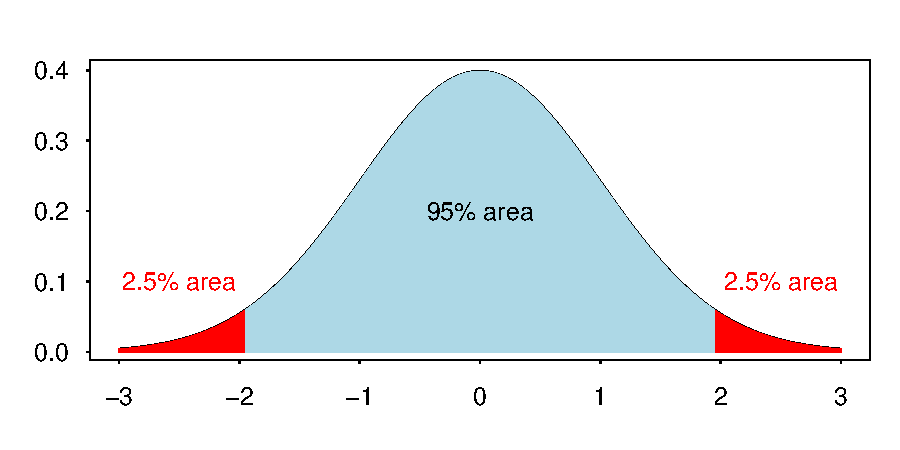
\includegraphics[width=\textwidth]{normal_areas.pdf}
\end{center}

\end{frame}

\begin{frame}[fragile]{}
\bbl{\Huge The $t$ distribution}\\ 
\vspace{0.5cm}
\end{frame}


\begin{frame}{Using Student's $t$-distribution instead}

\begin{itemize}
\item If we replace the population parameter and standard deviation values, we have:
$$\mbox{Standardised value} = \frac{\mbox{Sample statistic}-\mbox{Hypothesised population value}}{\mbox{sample standard error}}$$
\item If we knew the true standard error of the sample statistic, then the standardised value would be normally distributed. However, when we use the standard error we end up with something that is $t$-distributed
\item The $t$-distribution (or Student's $t$-distribution) is another bell-shaped distribution. It has an additional parameter to the Normal distribution called the \bre{degrees of freedom} (df). For most of the examples we meet the degrees of freedom parameter is a function of the sample size
\item When df$=\infty$ then the pdf of $t$ is equivalent to the normal distribution. When df is small, the bell shape has much longer tails
\end{itemize}
\end{frame}

\begin{frame}{Student's $t$-distribution: pictures}
\begin{center}
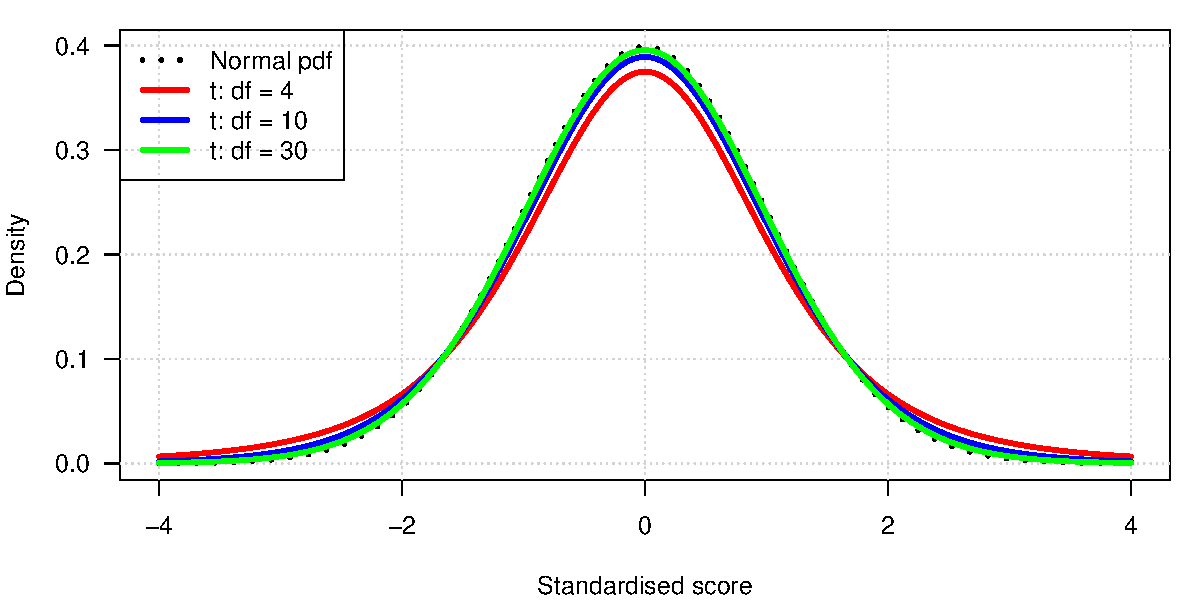
\includegraphics[width=\textwidth]{tdists.pdf}
\end{center}
We \bre{always} use the $t$-distribution when we don't know the true standard deviation of the sample statistic
\end{frame}

\begin{frame}{The law of large numbers and the central limit theorem}

There are two key statistical results that are relevant here:
\begin{enumerate}
\item The \bre{law of large numbers} states that \bgr{the sample mean will `eventually' get `close' to the population mean as the sample size rises}. This happens no matter how you define `close' though `eventually' could be a very long time
\pause
\item The \bre{central limit theorem} (CLT) is possibly the most important theorem in statistics. It states that \bgr{if the sample size is sufficiently large, the sample means of random samples from a population with some mean and standard deviation are approximately normally distributed with the same mean and standard deviation equal to the original standard deviation divided by the square root of the sample size}
\end{enumerate}
All of the results of the different situations we have met in this lecture follow from the CLT
\end{frame}

\begin{frame}[fragile]{}
\bbl{\Huge $t$-tests}\\ 
\vspace{0.5cm}
\end{frame}

\begin{frame}\frametitle{Example}
A random sample of 14 cows was selected from a large dairy herd in Cork. The milk yield in one week was recorded, in kg, for each cow. \\
\vspace{0.5cm}
\begin{tabular}{ccccccc}
169.6&142&103.3&111.6&123.4&143.5&155.1\\
101.7&170.7&113.2&130.9&146.1&169.3&155.5
\end{tabular}
\vspace{0.5cm}

\begin{itemize}
\item Dept. of Ag. want to investigate the farmer's claim that the mean weekly milk yield for the herd is 120kg.
\end{itemize}
\end{frame}


\begin{frame}\frametitle{Milk yield example}
\begin{enumerate}
\item[1] \emph{State the Null and Alternative Hypotheses ($H_0$ and $H_A$).}
$$H_{0}: \mbox{population mean} = 120 \mbox{ and } H_{A}: \mbox{population mean} \neq 120$$
\item[2] \emph{Identify the level of significance.}
$$\mbox{We will use } 0.05  = 5\%$$
\item[3] \emph{Assume $H_0$ is true and compute the test statistic. }
\begin{eqnarray*} 
\mbox{test statistic} & = &\frac{\mbox{sample mean} - 120}{\mbox{standard deviation}/\sqrt{n}} \\
 & & \\
 &=& \frac{138.278 - 120}{24.58/\sqrt{14}} \\
  & & \\
 & =& 2.78
\end{eqnarray*}
\end{enumerate}
\end{frame}

\begin{frame}
\frametitle{Milk yield example}
\begin{enumerate}
\item[4] \emph{Identify the rejection region: use the appropriate Excel function and significance level to find critical value(s).\\}
\end{enumerate}
$$\mbox{2 tailed test. } \hspace{0.5cm} df =  n - 1 = 13.$$ 
\vspace{-0.8cm}
\begin{center}
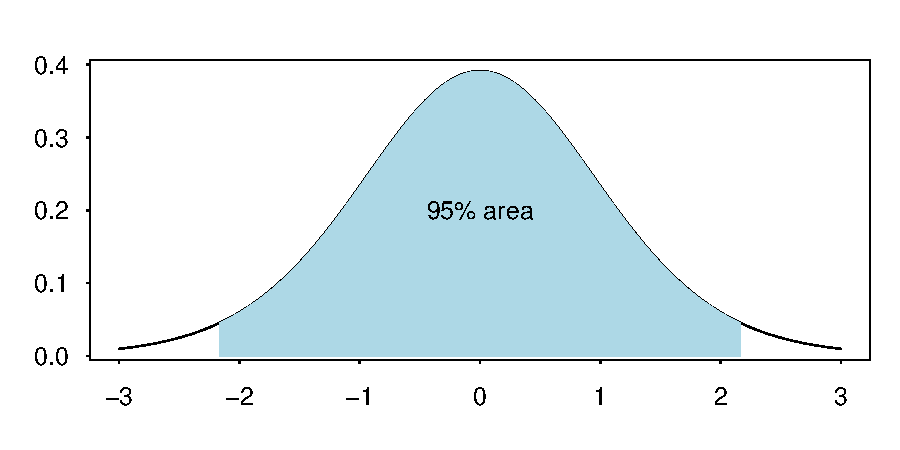
\includegraphics[width=0.7\textwidth]{t_plot.pdf}
\end{center}
$$\mbox{ critical value } = 2.16 \mbox{ (Excel formula was \texttt{T.INV.2T(0.05, 13)})}$$


\end{frame}

\begin{frame}\frametitle{Milk yield example}
\begin{enumerate}
\item[5] \emph{Compare the test statistic with the critical value(s).}
\begin{center}
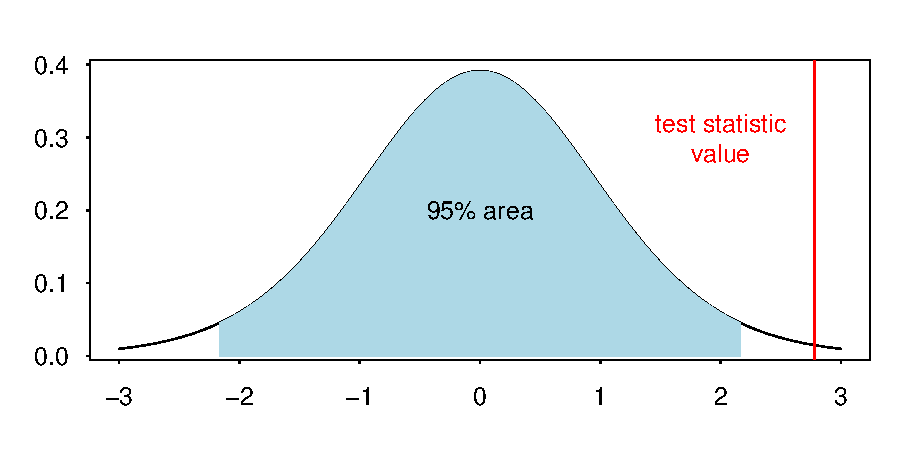
\includegraphics[width=0.8\textwidth]{t_plot2.pdf}
\end{center}
$$\mbox{test statistic } = 2.78 > 2.16 = \mbox{critical value}$$
    \end{enumerate}
\end{frame}

\begin{frame}\frametitle{Milk yield example}
\begin{enumerate}
\item[6] \emph{Draw a conclusion:}\\
\vspace{0.5cm}
Test statistic falls inside the rejection region so\\ reject $H_0$ and conclude that $H_A$ is true. \\
\item[7] \emph{Interpret the conclusion:}\\
\vspace{0.5cm}
The mean weekly milk yield is \emph{significantly different} from 120kgs, at the 5\% level.
    \end{enumerate}
\end{frame}

\begin{frame}
\frametitle{$p$-value approach to hypothesis testing}
\begin{itemize}
\item The conclusion of a hypothesis test is dependent on the choice of the significance level (usually 0.05).
\item Rather than pick a value, you could find the value associated with the test statistic value. This is the $p$-value approach we met yesterday.
\item The $p$-value can be compared to the significance level, so each person can make a decision based on their own choice of value. Excel usually provides the $p$-value for you
\end{itemize}
\end{frame}

\begin{frame}
\frametitle{$p$-value approach to hypothesis testing}
\begin{itemize}
\item Our test statistic value was 2.78. We can calculate the probability of being more extreme than this value using Excel
\item The formula is: 	\texttt{T.DIST.2T(2.78, 13)} = 0.016.
\item This is smaller than 0.05 so if using 5\% as the significance level we can say that the result is `statistically significant at the 1.6\% level'
\end{itemize}
\end{frame}

\begin{frame}{$p$-values continued}
\begin{itemize}
\item Don't forget what statistical significance means. It is not a measure of whether a result is large or important. It means that you have a big enough sample size to `signify' something
\item The American Statistical Association recently released some advice on $p$-values:
\end{itemize}
\begin{quote}
By itself, a p-value does not provide a good measure of evidence regarding a model or hypothesis\footnote{http://amstat.tandfonline.com/doi/pdf/10.1080/00031305.2016.1154108?needAccess=true}
\end{quote}
\end{frame}

\begin{frame}
\frametitle{Difference between two population means}
Many studies are undertaken with the objective of comparing the characteristics of two populations. In such cases we need two samples, one from each population.

\begin{block}{Examples}
\begin{itemize}
\item Compare the average fuel consumption of Volvo and Renault cars.
\item Compare the proportion of the population $<$ 25 yrs in the UK and Ireland.
\item Compare the average IQ for males and females.
\item Compare the proportion of people 'improved' following treatment for hayfever with drug A and drug B.
\end{itemize}
\end{block}
\end{frame}


\begin{frame}
\frametitle{Difference between two population means}
\begin{center}
{\small{
\begin{tabular}{cccc}
Population 1	&&& Population	2\\
Pop mean 1, Pop sd 1 &&& Pop mean 2, Pop sd 2\\
$\Downarrow$&&&$\Downarrow$\\
Sample 1	&&& Sample	2\\
Sample mean 1, Sample sd 1 &&& Sample mean 2, Sample sd 2\\
\end{tabular}}}
\end{center}

\vspace*{0.2cm}
We are not interested in the population means themselves but in their difference
\begin{block}{For example}
\begin{itemize}
\item $\mbox{pop mean 1} - \mbox{pop mean 2} = 0$ implies $\mbox{pop mean 1} = \mbox{pop mean 2}$
\item $\mbox{pop mean 1} - \mbox{pop mean 2} > 0$ implies $\mbox{pop mean 1} > \mbox{pop mean 2}$
\item $\mbox{pop mean 1} - \mbox{pop mean 2} < 0$ implies $\mbox{pop mean 1} < \mbox{pop mean 2}$
\end{itemize}
\end{block}

The two samples will be \textbf{\tcb{independent}} or dependent (\textbf{\tcb{paired}}) according to the design of the experiment/study
\end{frame}

\begin{frame}\frametitle{Independent and Paired samples}

\textbf{Independent:} if selection of items for one sample does not depend in any way on the selection for the other sample.

\vspace*{0.2cm}

\textbf{Paired:} items in the two samples are paired in some way.

\vspace*{0.2cm}
\begin{block}{Example -- Study to compare average IQ of males and females.}
\begin{itemize}
\item 2 independent samples -- select random sample of males and then a random sample of females.
\item 2 paired samples -- select a number of brother \& sister pairs and these make up the two samples.
\end{itemize}
\end{block}

We only consider inferences based on independent samples
\end{frame}

\begin{frame}
\frametitle{Performing the hypothesis test}
\begin{itemize}
\item To test $H_0: \mbox{population mean difference} = 0$, the test statistic is:
$$\mbox{test statistic} = \frac{\mbox{mean group 1} - \mbox{mean group 2}}{\sqrt{ \left( \frac{\mbox{sd1}^2}{n_1}+\frac{\mbox{sd2}^2}{n_2} \right) }} $$
where these are all calculate on the sample data
\item The critical value then comes from the $t$-distribution with a complicated formula for the degrees of freedom:
$$df = \frac{ \left( \frac{s_1^2}{n_1} + \frac{s_2^2}{n_2} \right)^2 }{ \frac{1}{n_1-1} \left( \frac{s_1^2}{n_1} \right)^2 + \frac{1}{n_2-1} \left( \frac{s_2^2}{n_2} \right)^2 } $$
\end{itemize}
\end{frame}


\begin{frame}
\frametitle{More advanced version.}
\begin{itemize}
\item To test the more complicated hypothesis: $$H_0: \mbox{population mean difference} = k$$
\item The test statistic is then:
$$\mbox{test statistic} = \frac{\mbox{mean group 1} - \mbox{mean group 2} - k}{\sqrt{ \left( \frac{\mbox{sd1}^2}{n_1}+\frac{\mbox{sd2}^2}{n_2} \right) }} $$
\item ... but everything else is the same
\end{itemize}
\end{frame}

\begin{frame}
\frametitle{Example - slow learners}
10 pupils previously diagnosed as slow learners were taught by a new method, 12 taught by a standard method. After 6 months they are scored on a reading test with the following results:
\begin{center}
{\small{
\begin{tabular}{|l|c|c|c|}\hline
& $n$ & $mean$ & $sd$ \\ \hline
New method	& 10 & 76.4 & 5.84 \\
Standard method 	& 12 & 72.3 & 6.34\\ \hline
\end{tabular}}}
\end{center}
\vspace*{0.4cm}
At the 5\% level, do these data indicate that the new method is better?
\end{frame}

\begin{frame}
\frametitle{Example - slow learners}
\begin{itemize}
\item $H_0: \mbox{population mean difference} = 0$ vs $H_A: \mbox{population mean difference} \ne 0$
\item Test statistic:
$$\mbox{test statistic} = \displaystyle\frac{(76.4 - 72.3)}{\sqrt{\frac{5.84^2}{10} + \frac{6.34^2}{12}}} = 1.58$$
\item Compute the degrees of freedom:
$$df = \frac{ \left( \frac{5.84^2}{10} + \frac{6.34^2}{12} \right)^2 }{ \frac{1}{10-1} \left( \frac{5.84^2}{10} \right)^2 + \frac{1}{12-1} \left( \frac{6.34^2}{12} \right)^2 } = 19.77$$
\item Compare with critical value 2.09 ( \texttt{T.INV.2T(0.05, 20)} in Excel)
\item Conclusion - do not reject $H_0$ at 5\% level
\vspace*{0.5cm}
\end{itemize}
\end{frame}

\begin{frame}[fragile]{}
\bbl{\Huge Confidence Intervals}\\ 
\vspace{0.5cm}
\end{frame}

\begin{frame}{Confidence intervals and confidence levels}

\begin{itemize}
\item A confidence interval is a set of two values (lower and upper) accompanied by a \bbl{confidence level}.
\item The confidence level tells us how likely it is that the interval estimate contains the true value of the parameter
\item Most commonly we calculate 90\%, 95\% and 99\% confidence intervals
\item As we are often assuming the sampling distribution to be normal (or $t$), we cannot calculate a 100\% confidence interval (remember that the bell-shaped normal distribution has infinite tails from our empirical rule)
\end{itemize}

\end{frame}

\begin{frame}{Interpreting confidence intervals}
\bre{BEWARE: this is something lots of people get wrong}
\begin{itemize}
\item Our confidence level quantifies how likely it is that the interval estimate contains the true value of the parameter
\item It does not tell us how likely the parameter is to be in the interval
\item This is because our parameters are \bre{fixed} and the uncertainty is in the \bgr{sample data}
\item A more complete definition is that a 95\% confidence interval would include the true population value for 95\% of all possible random samples from the population
\end{itemize}

\end{frame}

\begin{frame}{How to calculate confidence intervals}

\begin{block}{}
A confidence interval or interval estimate (in all of the situations we meet) can be calculated as:
$$\mbox{Sample estimate} \pm \mbox{Multiplier} \times \mbox{Standard error}$$
The multiplier is based on the confidence level desired and the probability distribution 
\end{block}
\pause
\begin{itemize}
\item Here the \bbl{sample estimate} is the statistic we can calculate from the sample data
\item The \bgr{multiplier} determines the amount of confidence we will have in the result
\item The \bre{standard error} is the standard error of the statistic we are trying to calculate
\end{itemize}
\end{frame}

\begin{frame}{A CI for a single population mean}
The confidence interval for a single population mean is:
$$\mbox{sample mean} \pm \mbox{t-value} \frac{\mbox{standard deviation}}{\sqrt{\mbox{sample size}}}$$
Some notes:
\begin{itemize}
\item $\frac{\mbox{standard deviation}}{\sqrt{\mbox{sample size}}}$ is our estimate of the standard error of the mean
\item The $t$-value is the multiplier for the $t$-distribution with $(\mbox{sample size}-1)$ degrees of freedom at the chosen confidence level
\item We use the $t$ distribution here because the normal distribution is invalid when the sample size is small. When the sample size is large the $t$ and the normal are the same
\end{itemize}
\end{frame}

\begin{frame}\frametitle{Example}
A random sample of 14 cows was selected from a large dairy herd in Cork. The milk yield in one week was recorded, in kg, for each cow. \\
\vspace{0.5cm}
\begin{tabular}{ccccccc}
169.6&142&103.3&111.6&123.4&143.5&155.1\\
101.7&170.7&113.2&130.9&146.1&169.3&155.5
\end{tabular}
\vspace{0.5cm}

\begin{enumerate}
\item Dept. of Ag. want to investigate the farmer's claim that the mean weekly milk yield for the herd is 120kg. Create a 95\% confidence interval for the mean weekly milk yield.
\end{enumerate}
\end{frame}


\begin{frame}\frametitle{Milk yield example}
\underline{Small Sample CI:}\\
$$\mbox{sample mean} \pm (\mbox{$t$ value}) \frac{\mbox{standard deviation}}{\sqrt{n}}$$
\begin{eqnarray*}
138.28 & \pm & (2.16) \frac{24.58}{\sqrt{14}}\\
\end{eqnarray*}
$$(124.09, 152.47)$$
Based on our sample, we are 95\% confident that the mean weekly milk yield lies between 124kg and 152kg.
\end{frame}

\begin{frame}{Where did the $t$-value come from?}

\begin{itemize}
\item In the previous slide we used 2.16 as the $t$-value in the confidence interval. 
\item This value is the 97.5th percentile of the $t$-distribution with 13 degrees of freedom
\item For a 99\% confidence interval we would use the 99.5th percentile of the $t$-distribution. (It always helps to draw a picture)
\item In Excel, we'd use \texttt{T.INV(0.975, 13)} which will return the value 2.16
\end{itemize}

\end{frame}

\begin{frame}{$t$-value picture}
\begin{center}
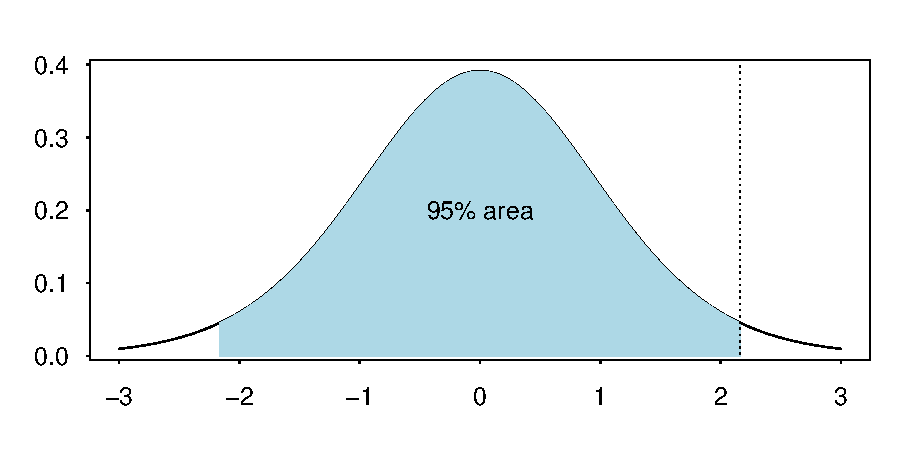
\includegraphics[width=\textwidth]{t_plot3.pdf}
\end{center}

\end{frame}

\begin{frame}{ What determines the width of a CI?}

Three things determine the width of a confidence interval:
\begin{enumerate}
\item The sample size $n$. If $n$ is large we will have a smaller interval because the standard error will be smaller
\item The confidence level. The more confident we want to be the wider we have to make the interval
\item The natural variability of the data. If the data are very variable then our confidence interval will be wider
\end{enumerate}
Note that we have some control over (1) and (2) but no control over (3)
\end{frame}

\begin{frame}{CI for the difference between two independent population means}

Suppose have two groups and want to calculate a confidence interval for the differences between them. We use the formula:

$$\mbox{mean group 1} - \mbox{mean group 2} \pm \mbox{$t$-value}\sqrt{ \left( \frac{\mbox{sd1}^2}{n_1}+\frac{\mbox{sd2}^2}{n_2} \right) }$$
where sd1 and sd2 are the standard deviations of each of the groups, as $n_1$ and $n_2$ are their sample sizes. \\
\vspace{0.5cm}
The extra complication in this version is that the $t$-value is harder to calculate
\end{frame}

\begin{frame}{Example}

\begin{block}{}
Some researchers were interested in the effect of hangovers amongst college students. Students were asked whether their parents suffered from alcohol problems and asked to rate the severity and duration of their own hangovers on a 13-point scale, with 13 being the most severe. 1227 students were contacted and the data are shown below. Calculate a 95\% confidence interval.
\begin{center}
\begin{tabular}{lccc}
\hline
Group & Sample & Mean & Standard \\
& size & & deviation \\
\hline
Parental alcohol problems & $n_1=282$ & $\mbox{mean grp 1}=5.9$ & $\mbox{sd1}=3.6$\\ 
No parental alcohol problems & $n_2=945$ & $\mbox{mean grp 2}=4.9$ & $\mbox{sd2}=3.4$\\
\hline
\end{tabular}
\end{center}
\end{block}
\end{frame}

\begin{frame}{Solution: using unequal variances}

This is the formula for the degrees of freedom (yikes!):
\begin{eqnarray*}
df = \frac{ \left( \frac{s_1^2}{n_1} + \frac{s_2^2}{n_2} \right)^2 }{ \frac{1}{n_1-1} \left( \frac{s_1^2}{n_1} \right)^2 + \frac{1}{n_2-1} \left( \frac{s_2^2}{n_2} \right)^2 } &=& \frac{ \left( \frac{3.6^2}{282} + \frac{3.4^2}{945} \right)^2 }{ \frac{1}{282-1} \left( \frac{3.6^2}{282} \right)^2 + \frac{1}{945-1} \left( \frac{3.4^2}{945} \right)^2 } \\
&\approx& 441 
\end{eqnarray*}
We also need 
$$\sqrt{ \left( \frac{s_1^2}{n_1}+\frac{s_2^2}{n_2} \right) } = \sqrt{ \left( \frac{3.6^2}{282}+\frac{3.4^2}{945} \right) } = 0.24$$
Finally we need \texttt{T.INV(0.975, 441)}$=1.96$ so the 95\% CI is:
\begin{block}{}
$$5.9-4.9 \pm 1.96 \times 0.24 = (0.53,1.47)\; \mbox{symptoms}$$
\end{block}
\end{frame}

\begin{frame}{Summary of class 4}
\begin{itemize}
\item The $t$-distribution is the one to use whenever we don't know what the population standard deviation is (i.e. nearly always)
\item $t$-tests are created following the standard hypothesis testing steps. We calculate whether our test statistic is in the rejection region or not, or use a $p$-value
\item More useful than a hypothesis test is a confidence interval, which expresses uncertainty about how likely repeated samples are to contain the true value
\item 2-sample $t$-tests can be run in Excel through the Data Analysis package, whilst confidence intervals are not provided
\end{itemize}
\end{frame}

\end{document}
